\documentclass[aspectratio=169]{beamer}
\usetheme{Madrid}
\usecolortheme{default}

% Packages
\usepackage{graphicx}
\usepackage{amsmath}
\usepackage{amssymb}
\usepackage{tikz}
\usetikzlibrary{arrows,shapes,positioning,calc}
\usepackage{booktabs}
\usepackage{hyperref}

\graphicspath{{./}}

% Custom colors
\definecolor{primary}{RGB}{10,37,64}
\definecolor{secondary}{RGB}{99,91,255}
\definecolor{accent}{RGB}{0,212,255}
\definecolor{success}{RGB}{50,213,131}
\definecolor{warning}{RGB}{255,193,7}
\definecolor{danger}{RGB}{220,53,69}

\setbeamercolor{structure}{fg=secondary}
\setbeamercolor{palette primary}{bg=primary,fg=white}
\setbeamercolor{palette secondary}{bg=secondary,fg=white}
\setbeamercolor{palette tertiary}{bg=accent,fg=white}

% Title page
\title[SE446 - Week 1]{Course Introduction}
\subtitle{Big Data Analytics}
\author{Professor Anis Koubaa}
\institute{
    SE 446\\
    Alfaisal University\\[0.3em]
    \url{https://github.com/aniskoubaa/big_data_course}
}
\date{Spring 2026}
\titlegraphic{\includegraphics[width=1.5cm]{logo.png}}

% ============================================
% BEGIN DOCUMENT
% ============================================
\begin{document}

% Title slide
\begin{frame}
\titlepage
\end{frame}

% Outline
\begin{frame}{Outline}
  \tableofcontents[hideallsubsections]
\end{frame}

% ===========================================
\section{Welcome \& Course Overview}
% ===========================================

\begin{frame}{Welcome to SE 446!}
  \begin{columns}[T]
    \begin{column}{0.55\textwidth}
      \begin{block}{Course Info}
        \begin{itemize}
          \item \textbf{Credits}: 3 hours
          \item \textbf{Duration}: 13 weeks
          \item \textbf{Schedule}: 2 sessions/week
        \end{itemize}
      \end{block}
      
      \vspace{0.5em}
      
      \begin{block}{Instructor}
        \begin{itemize}
          \item Prof. Anis Koubaa
          \item \texttt{akoubaa@alfaisal.edu}
          \item Office: SG-10
        \end{itemize}
      \end{block}
    \end{column}
    
    \begin{column}{0.4\textwidth}
      \centering
      \includegraphics[width=0.5\textwidth]{logo.png}
    \end{column}
  \end{columns}
\end{frame}

\begin{frame}{What is Big Data?}
  \begin{block}{Definition}
    Data that is too \textcolor{secondary}{\textbf{large}}, \textcolor{success}{\textbf{fast}}, or \textcolor{warning}{\textbf{complex}} for traditional tools to process.
  \end{block}
  
  \vspace{0.5em}
  
  \begin{columns}[T]
    \begin{column}{0.48\textwidth}
      \textbf{Scale Examples:}
      \begin{itemize}
        \item Facebook: 4 PB/day
        \item YouTube: 500 hrs video/min
        \item Twitter: 500M tweets/day
        \item Google: 20 PB processed/day
      \end{itemize}
    \end{column}
    
    \begin{column}{0.48\textwidth}
      \textbf{Why It Matters:}
      \begin{itemize}
        \item Better business decisions
        \item Scientific discoveries
        \item Real-time insights
        \item Competitive advantage
      \end{itemize}
    \end{column}
  \end{columns}
\end{frame}

\begin{frame}{Course Learning Outcomes (CLOs)}
  By the end of this course, you will be able to:
  
  \vspace{0.3em}
  
  \begin{enumerate}
    \item \textbf{Knowledge \& Understanding}
    \begin{itemize}
      \item Explain essential concepts, challenges, and approaches in Big Data
    \end{itemize}
    
    \vspace{0.2em}
    
    \item \textbf{Skills}
    \begin{itemize}
      \item Implement scalable data processing pipelines for batch, streaming, and distributed real-time workflows on distributed platforms
    \end{itemize}
    
    \vspace{0.2em}
    
    \item \textbf{Perform Data Analysis}
    \begin{itemize}
      \item Perform data analysis on large datasets and interpret results to support evidence-based decision making in real-world contexts
    \end{itemize}
    
    \vspace{0.2em}
    
    \item \textbf{Values, Autonomy, \& Responsibility}
    \begin{itemize}
      \item Demonstrate ethical, responsible, and collaborative practices when working with data, including respect for privacy, security, and teamwork principles
    \end{itemize}
  \end{enumerate}
\end{frame}

% ===========================================
\section{Course Logistics}
% ===========================================

\begin{frame}{Weekly Schedule}
  \centering
  \begin{tabular}{clll}
    \toprule
    \textbf{Week} & \textbf{Topic} & \textbf{Milestone} & \textbf{Assessment} \\
    \midrule
    1 & Course Introduction & -- & -- \\
    2 & Big Data + HDFS & -- & -- \\
    3-4 & Data Formats + MapReduce & M1 & -- \\
    5-6 & Hive + M2 & M2 & \textcolor{danger}{Midterm 1} \\
    7-8 & Apache Spark & M3 & -- \\
    9-10 & Kafka + Streaming + M4 & M4 & \textcolor{danger}{Midterm 2} \\
    11-12 & Project Completion & M5 & Quiz 1, 2 \\
    13 & Final Review & -- & -- \\
    \bottomrule
  \end{tabular}
\end{frame}

\begin{frame}{Grading Breakdown}
  \begin{columns}[T]
    \begin{column}{0.5\textwidth}
      \centering
      \begin{tabular}{lr}
        \toprule
        \textbf{Component} & \textbf{Weight} \\
        \midrule
        Midterm 1 & 20\% \\
        Midterm 2 & 20\% \\
        Final Exam & 30\% \\
        Quizzes (2) & 10\% \\
        Project Work & 20\% \\
        \midrule
        \textbf{Total} & \textbf{100\%} \\
        \bottomrule
      \end{tabular}
    \end{column}
    
    \begin{column}{0.45\textwidth}
      \begin{block}{Project Work (20\%)}
        \textbf{5 Milestones} (4\% each)
        
        \vspace{0.5em}
        \textbf{What counts:}
        \begin{itemize}
          \item Github commits
          \item Regular submissions
          \item Milestone Quality
        \end{itemize}
      \end{block}
    \end{column}
  \end{columns}
\end{frame}

\begin{frame}{Attendance Policy}
  \begin{block}{Important}
    Attendance is \textbf{mandatory} and missing classes would affect your grades.
  \end{block}
  
  \vspace{0.5em}
  
  \begin{itemize}
    \item Each class has an in-class Moodle quiz (last 15 min)
    \item Missing an in-class submission will affect your grade
    \item Medical/official excuses within 48 hours
  \end{itemize}
\end{frame}

% ===========================================
\section{Tools \& Platforms}
% ===========================================

\begin{frame}{Tools We'll Use}
  \centering
  \begin{tabular}{lll}
    \toprule
    \textbf{Tool} & \textbf{Purpose} & \textbf{Weeks} \\
    \midrule
    Google Colab & Python, Pandas, PySpark basics & 1-4 \\
    Databricks & Spark, Hive, Streaming & 5-10 \\
    VS Code & Local development (optional) & All \\
    GitHub & Code collaboration & All \\
    Moodle & In-class quizzes & All \\
    \bottomrule
  \end{tabular}
  
  \vspace{1em}
  
  \begin{block}{No Installation Required!}
    Everything runs in the \textbf{cloud}. You only need a web browser.
  \end{block}
\end{frame}

\begin{frame}{Google Colab \& Databricks}
  \begin{columns}[T]
    \begin{column}{0.48\textwidth}
      \begin{block}{Google Colab}
        \begin{itemize}
          \item Free Jupyter notebooks in the cloud
          \item Python + libraries pre-installed
          \item Easy sharing via Google Drive
          \item GPU access when needed
        \end{itemize}
        \textbf{URL:} \url{colab.google.com}
      \end{block}
    \end{column}
    
    \begin{column}{0.48\textwidth}
      \begin{block}{Databricks Community}
        \begin{itemize}
          \item Free cloud Big Data platform
          \item Apache Spark pre-configured
          \item Industry-standard tool
          \item Notebooks + cluster management
        \end{itemize}
        \textbf{URL:} \url{databricks.com/try}
      \end{block}
    \end{column}
  \end{columns}
\end{frame}

% ===========================================
\section{Semester Project}
% ===========================================

\begin{frame}{Project: Smart City Data Platform}
  \begin{block}{Concept}
    Build a data analytics platform using real urban datasets.
  \end{block}
  
  \vspace{0.5em}
  
  \centering
  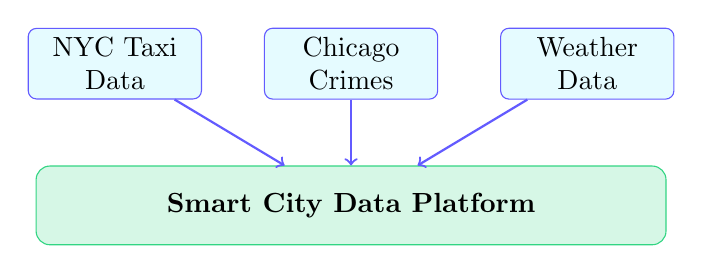
\begin{tikzpicture}[
    box/.style={rectangle, draw=secondary, fill=accent!10, 
                minimum width=2.2cm, minimum height=0.8cm, align=center, rounded corners=3pt},
    platform/.style={rectangle, draw=success, fill=success!20, 
                     minimum width=8cm, minimum height=1cm, align=center, rounded corners=5pt}
  ]
    \node[box] (taxi) at (-3, 0) {NYC Taxi\\Data};
    \node[box] (crime) at (0, 0) {Chicago\\Crimes};
    \node[box] (weather) at (3, 0) {Weather\\Data};
    
    \node[platform] (platform) at (0, -1.8) {\textbf{Smart City Data Platform}};
    
    \draw[->, thick, secondary] (taxi) -- (platform);
    \draw[->, thick, secondary] (crime) -- (platform);
    \draw[->, thick, secondary] (weather) -- (platform);
  \end{tikzpicture}
\end{frame}

\begin{frame}{5 Milestones}
  \centering
  \begin{tabular}{clcc}
    \toprule
    \textbf{M} & \textbf{Topic} & \textbf{Week Due} & \textbf{Weight} \\
    \midrule
    M1 & Data Loading (HDFS concepts) & 4 & 4\% \\
    M2 & MapReduce Processing & 6 & 4\% \\
    M3 & Hive Analytics & 8 & 4\% \\
    M4 & Spark Analysis & 10 & 4\% \\
    M5 & Streaming Pipeline & 12 & 4\% \\
    \midrule
    & \textbf{Total} & & \textbf{20\%} \\
    \bottomrule
  \end{tabular}
  
  \vspace{0.5em}
  
  \begin{block}{Per Milestone}
    \textbf{GitHub Commits} and \textbf{Related Assessment} will be counted towards project grade
  \end{block}
\end{frame}

\begin{frame}{Datasets We'll Use}
  \centering
  \begin{tabular}{lll}
    \toprule
    \textbf{Dataset} & \textbf{Size} & \textbf{Description} \\
    \midrule
    NYC Yellow Taxi & $\sim$50 MB & Trip records, fares, locations \\
    Chicago Crimes & $\sim$30 MB & Crime types, dates, locations \\
    NYC Weather & $\sim$5 MB & Daily temperature, precipitation \\
    Air Quality Index & $\sim$3 MB & Daily AQI by city \\
    \bottomrule
  \end{tabular}
  
  \vspace{0.5em}
  
  \begin{block}{Good News!}
    All datasets are pre-hosted. No downloading required.
  \end{block}
\end{frame}

% ===========================================
\section{GitHub Workflow}
% ===========================================

\begin{frame}{Course Repository}
  \begin{block}{GitHub Repository}
    \centering
    \Large\url{https://github.com/aniskoubaa/big_data_course}
  \end{block}
  
  \vspace{0.5em}
  
  \begin{itemize}
    \item All course materials (slides, notebooks, data)
    \item Weekly updates
    \item Milestone templates
    \item Clone it to get started!
  \end{itemize}
  
  \vspace{0.3em}
  
  \begin{block}{Clone Command}
    \texttt{git clone https://github.com/aniskoubaa/big\_data\_course.git}
  \end{block}
\end{frame}

\begin{frame}{Team Repository Structure}
  \begin{columns}[T]
    \begin{column}{0.5\textwidth}
      \textbf{Repository Organization:}
      
      \vspace{0.5em}
      
      Each team gets \textbf{ONE shared repository}
      
      \vspace{0.5em}
      
      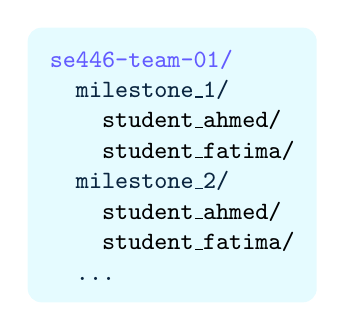
\begin{tikzpicture}[font=\ttfamily\small]
        \node[align=left, fill=accent!10, rounded corners=5pt, inner sep=8pt] at (0,0) {
          \textcolor{secondary}{\textbf{se446-team-01/}}\\
          ~~\textcolor{primary}{milestone\_1/}\\
          ~~~~student\_ahmed/\\
          ~~~~student\_fatima/\\
          ~~\textcolor{primary}{milestone\_2/}\\
          ~~~~student\_ahmed/\\
          ~~~~student\_fatima/\\
          ~~\textcolor{primary}{...}
        };
      \end{tikzpicture}
    \end{column}
    
    \begin{column}{0.45\textwidth}
      \textbf{Important Rules:}
      \begin{itemize}
        \item Each student works in their \textbf{own folder}
        \item Individual commits are tracked separately
        \item Work on your assigned tasks only
        \item Quality matters more than quantity
      \end{itemize}
      
      \vspace{0.5em}
      
      \begin{block}{Note}
        \small Your individual contributions will be evaluated based on your folder's commits
      \end{block}
    \end{column}
  \end{columns}
\end{frame}

\begin{frame}{Git Workflow (Simplified)}
  \centering
  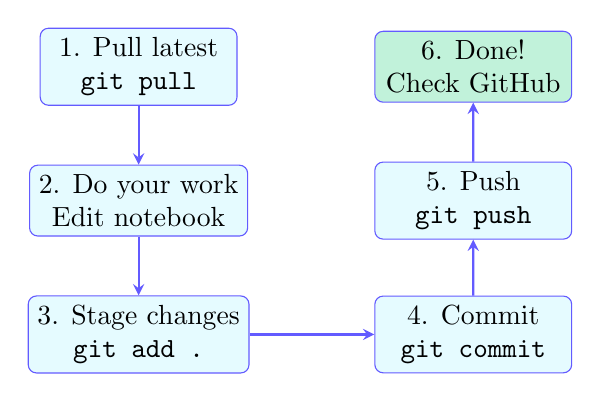
\begin{tikzpicture}[
    workflowstep/.style={rectangle, draw=secondary, fill=accent!10, 
                 minimum width=2.5cm, minimum height=0.9cm, align=center, rounded corners=3pt},
    arr/.style={->, >=stealth, thick, secondary},
    scale=0.85
  ]
    \node[workflowstep] (pull) at (0, 2)    {1. Pull latest\\\ttfamily git pull};
    \node[workflowstep] (work) at (0, 0)    {2. Do your work\\Edit notebook};
    \node[workflowstep] (add) at (0, -2)    {3. Stage changes\\\ttfamily git add .};
    \node[workflowstep] (commit) at (5, -2) {4. Commit\\\ttfamily git commit};
    \node[workflowstep] (push) at (5, 0)    {5. Push\\\ttfamily git push};
    \node[workflowstep, fill=success!30] (done) at (5, 2) {6. Done!\\Check GitHub};
    
    \draw[arr] (pull) -- (work);
    \draw[arr] (work) -- (add);
    \draw[arr] (add) -- (commit);
    \draw[arr] (commit) -- (push);
    \draw[arr] (push) -- (done);
  \end{tikzpicture}
\end{frame}

\begin{frame}{Commit Message Standards}
  \begin{block}{Format}
    \texttt{<MILESTONE>: <Short description>}
  \end{block}
  
  \vspace{0.5em}
  
  \textbf{Good Examples:}
  \begin{itemize}
    \item \texttt{M1: Loaded NYC taxi data and checked schema}
    \item \texttt{M2: Implemented mapper for crime type count}
    \item \texttt{M3: Added HiveQL query for average fare}
  \end{itemize}
  
  \vspace{0.5em}
  
  \textbf{Bad Examples:}
  \begin{itemize}
    \item \texttt{update} $\leftarrow$ Too vague
    \item \texttt{asdfasdf} $\leftarrow$ Meaningless
  \end{itemize}
\end{frame}

% ===========================================
\section{Summary \& Next Steps}
% ===========================================

\begin{frame}{Summary}
  \begin{enumerate}
    \item \textbf{Course}: Learn Big Data processing with Hadoop, Spark, Kafka
    \item \textbf{Grading}: Exams (70\%) + Quizzes (10\%) + Project (20\%)
    \item \textbf{Tools}: Colab, Databricks, VS Code, GitHub, Moodle
    \item \textbf{Project}: 5 milestones with real urban datasets
    \item \textbf{GitHub}: Your commits are tracked and analyzed
  \end{enumerate}
  
  \vspace{0.5em}
  
  \begin{block}{Course Repository}
    \url{https://github.com/aniskoubaa/big_data_course}
  \end{block}
\end{frame}

\begin{frame}{Action Items for This Week}
  \begin{enumerate}
    \item \textbf{Create accounts} (if you don't have):
      \begin{itemize}
        \item GitHub: \url{github.com}
        \item Google (for Colab): \url{google.com}
      \end{itemize}
    \item \textbf{Clone the course repository}
    \item \textbf{Watch pre-class video} for Week 2:
      \begin{itemize}
        \item ``What is Big Data?'' - Simplilearn ($\sim$15 min)
      \end{itemize}
  \end{enumerate}
\end{frame}

\begin{frame}{Next Week Preview}
  \begin{block}{Week 2: Introduction to Big Data \& HDFS}
    \begin{itemize}
      \item The 5 V's of Big Data
      \item HDFS Architecture
      \item File Formats (CSV, JSON, Parquet)
      \item First hands-on notebook!
    \end{itemize}
  \end{block}
  
  \vspace{0.5em}
  
  \centering
  \textit{Get ready to dive into Big Data!}
\end{frame}

\begin{frame}{}
  \centering
  \vspace{2em}
  
  {\Huge\textcolor{secondary}{\textbf{Questions?}}}
  
  \vspace{1.5em}
  
  {\Large Let's set up your accounts!}
  
  \vspace{1em}
  
  Prof. Anis Koubaa\\
  \texttt{akoubaa@alfaisal.edu}\\[0.5em]
  \url{https://github.com/aniskoubaa/big_data_course}
\end{frame}

\end{document}
